\documentclass[aspectratio=169,10pt]{beamer}
\usetheme{default}
\setbeamercovered{invisible}
\setbeamertemplate{navigation symbols}{}
\setbeamertemplate{footline}{
    \flushright{\hfill \insertframenumber{}/\inserttotalframenumber}
}

\usepackage{listings}
\lstset{language=C++,
	basicstyle=\ttfamily,
	keywordstyle=\color{blue}\ttfamily,
	stringstyle=\color{red}\ttfamily,
	commentstyle=\color{green}\ttfamily,
	morecomment=[l][\color{magenta}]{\#}
}


% User-defined colors.
\definecolor{DarkGreen}{rgb}{0, .5, 0}
\definecolor{DarkBlue}{rgb}{0, 0, .5}
\definecolor{DarkRed}{rgb}{.5, 0, 0}
\definecolor{LightGray}{rgb}{.95, .95, .95}
\definecolor{White}{rgb}{1.0,1.0,1.0}
\definecolor{darkblue}{rgb}{0,0,0.9}
\definecolor{darkred}{rgb}{0.8,0,0}
\definecolor{darkgreen}{rgb}{0.0,0.85,0}

% Settings for listing class.
\lstset{
  language=C++,                        % The default language
  basicstyle=\small\ttfamily,          % The basic style
  backgroundcolor=\color{White},       % Set listing background
  keywordstyle=\color{DarkBlue}\bfseries, % Set keyword style
  commentstyle=\color{DarkGreen}\itshape, % Set comment style
  stringstyle=\color{DarkRed}, % Set string constant style
  extendedchars=true % Allow extended characters
  breaklines=true,
  basewidth={0.5em,0.4em},
  fontadjust=true,
  linewidth=\textwidth,
  breakatwhitespace=true,
  showstringspaces=false,
  lineskip=0ex, %  frame=single
}

\begin{document}
    \title{A complete Newton solver using \texttt{Eigen}}
    \author
      {
      Alberto Artoni
      }
    \date{April 05, 2024}

\begin{frame}[plain, noframenumbering]
    \maketitle
    
\end{frame}


\begin{frame}{Newton solver}
This example (an extended version of \texttt{Examples/src/NewtonSolver}) is about a set of tools that implement generic Newton or quasi-Newton methods to determine the zero of scalar non-linear equations, as well as vector systems using the \texttt{Eigen} library.

\end{frame}

\begin{frame}{Newton solver}
The code structure is the following:
\begin{itemize}
\item \texttt{NewtonTraits} contains the definition of the types used by the main classes, to guarantee uniformity.
\item \texttt{JacobianBase} is a base class which implements the action of a \textit{quasi-Jacobian}: the user may choose among \texttt{FullJacobian} where the actual Jacobian must be specified by the user, and \texttt{DiscreteJacobian}, that approximates the Jacobian via finite differences.
\item \texttt{JacobianFactory} instantiates a concrete derived class of \texttt{JacobianBase} family on the fly.
\item \texttt{Newton} applies the Newton method, given the non-linear system and a \texttt{JacobianBase}.
\item \texttt{NewtonOptions} and \texttt{NewtonResults} bind the input options and the output results.
\end{itemize}
\end{frame}

\begin{frame}{Abstract Class}
	\texttt{JacobianBase} is a base class which implements the action of a \textit{quasi-Jacobian}:
\begin{itemize}
	\item \texttt{FullJacobian}: the Jacobian must be specified by the user.
	\item \texttt{DiscreteJacobian}: the Jacobian is approximated via finite differences.	
\end{itemize}
	
	\begin{center}
	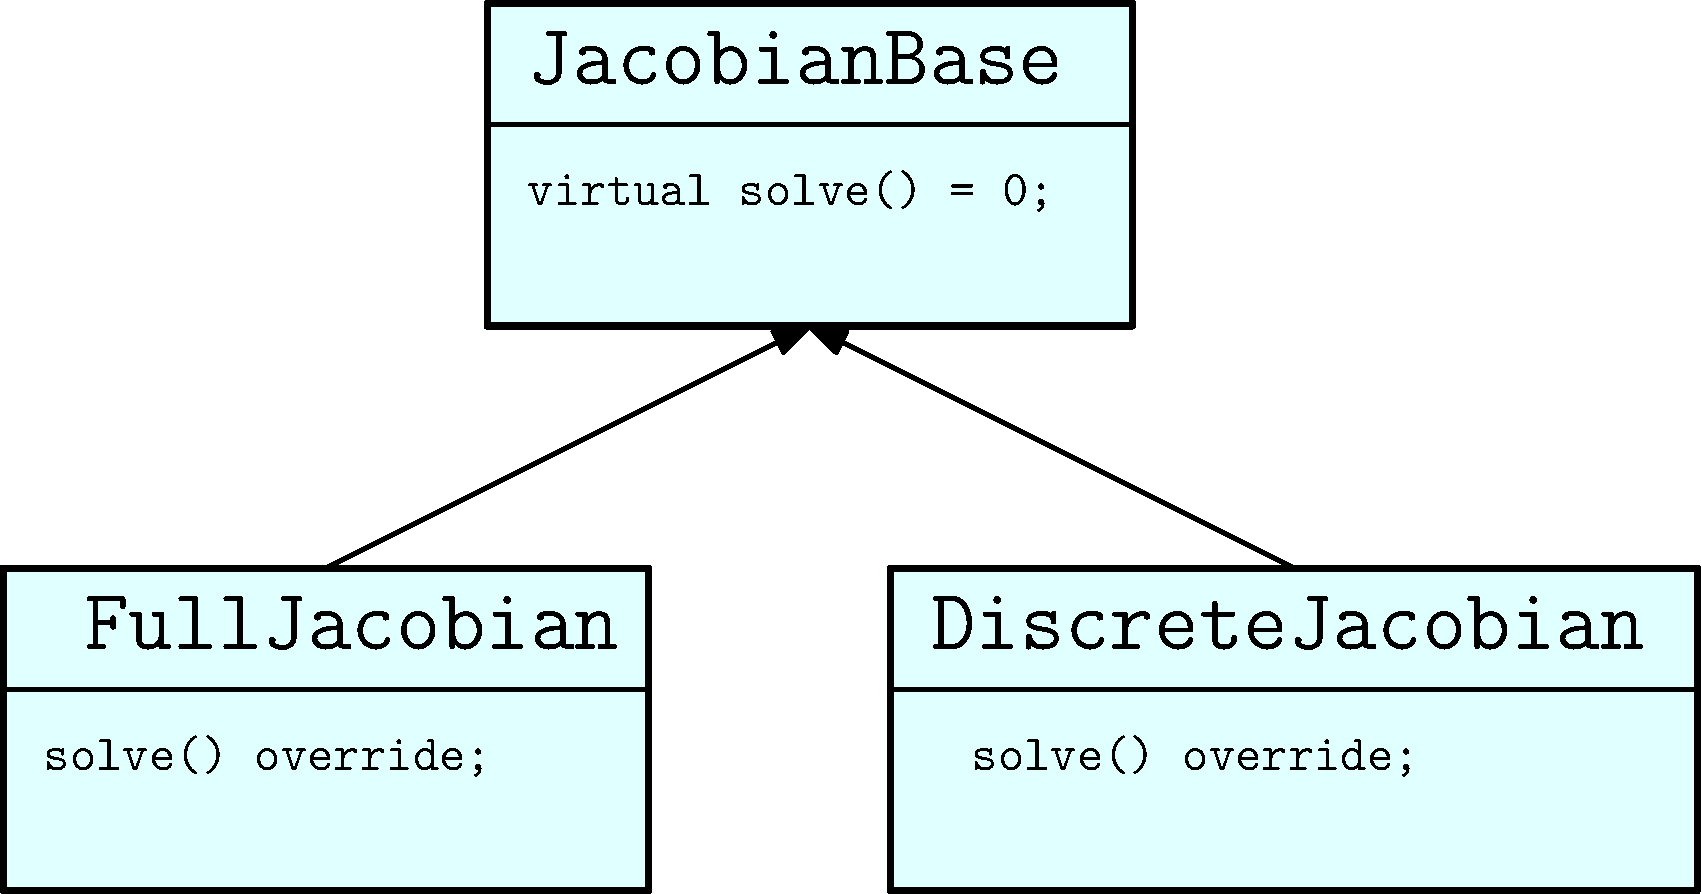
\includegraphics[width=0.35\textwidth]{ipe/class.pdf}
	\end{center}
\end{frame}

\begin{frame}[fragile]{Smart Pointers}
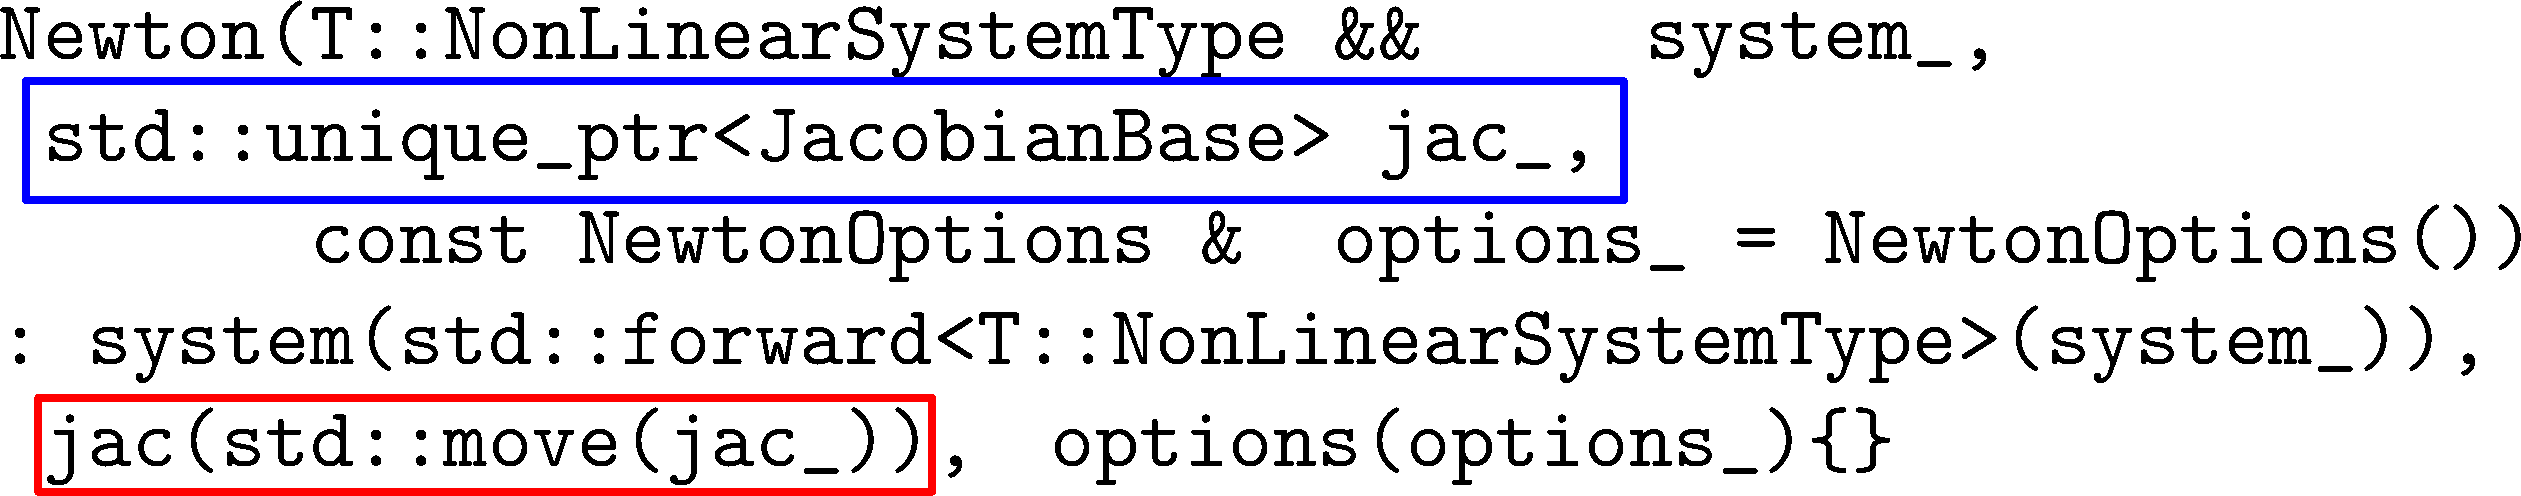
\includegraphics[width=0.65\textwidth]{ipe/newton.pdf}

The \texttt{Newton} class is initialized with a smart pointer to the \texttt{JacobianBase} class. Recall that since is an abstract class, we cannot instantiate an object. Hence we must use pointers. \\

Move semantic will be detailed later from the professor.
\end{frame}


\begin{frame}{Exercise}
Consider the problem
\[
\mathbf{f}(x, y) =
\begin{bmatrix}
(x-1)^2 + 0.1(y - 5)^2 \\
1.5 -x - 0.1y
\end{bmatrix}
=
\mathbf{0}.
\]

Starting from the provided solution sketch:
\begin{enumerate}
\item Implement the \texttt{NewtonTraits} class defining common types for homogeneity.
\item Implement the \texttt{FullJacobian} class (inheriting from \texttt{JacobianBase}) which, provided the full Jacobian matrix, solves the linear system using a direct solver with \(LU\) factorization.
\item \texttt{DiscreteJacobian} (inheriting from \texttt{JacobianBase}) which approximates the system Jacobian using finite differences and solves the linear system using a direct solver with \(LU\) factorization.
\item Implement a \texttt{JacobianFactory} method, returning an istance of \texttt{FullJacobian} or \texttt{DiscreteJacobian} depending on a parameter chosen by the user.
\item Solve the problem above using both the full and the discrete approach.
\end{enumerate}
\end{frame}

\end{document}
